A key assumption in economics is that agents are fully informed. However, information is rarely available for free. Information costs can take many forms, time, cognitive effort, monetary expenditures, technological hurdles, and are ubiquitous in decision settings \citep{jessoeKnowledgeLessPower2014, tiefenbeckOvercomingSalienceBias2018}. In the context of electricity, monthly or yearly bills aggregate total consumption without detailing the energy use of specific services, making it difficult for households to assess the marginal costs of their actions.  \\

In this section, we extend a standard consumer theory model to introduce the impact of salience bias on decision-making, following the approach of \citet{alcocerSalienceBiasFramework2024}. From this framework, we derive our predictions and show why households may overconsume electricity, when the costs of consumption are not salient.

\subsection{Without Salience Bias}

An agent chooses a consumption bundle \( \mathbf{x} = (e, x) \in \mathbb{R}_+^2 \) to maximize utility \( u(e, x) \), where \( e \) denotes electricity consumption and \( x \) is a composite good. The utility function \( u : \mathbb{R}_+^2 \rightarrow \mathbb{R} \) is assumed to be strictly quasiconcave and strictly increasing in both arguments.\\

The agent solves:
\[
\max_{(e, x) \in \mathbb{R}_+^2} \quad u(e, x) \quad \text{s.t.} \quad p_e e + p_x x \leq w,
\]
where \( p_e > 0 \) and \( p_x > 0 \) denote prices of electricity and the composite good, and \( w > 0 \) is the agent’s wealth. Since utility is strictly increasing and prices are positive, the constraint binds. Let the unique solution be \( (e^*, x^*) \). \\

Figure~\ref{fig:Theory}a illustrates this scenario: the household selects the utility-maximizing bundle \( (e^*, x^*) \) on the budget line, achieving the highest attainable utility level \( u^* \). 


\begin{figure}[H]
    \centering
   
    
    \begin{subfigure}[b]{0.75\textwidth}
        \centering
        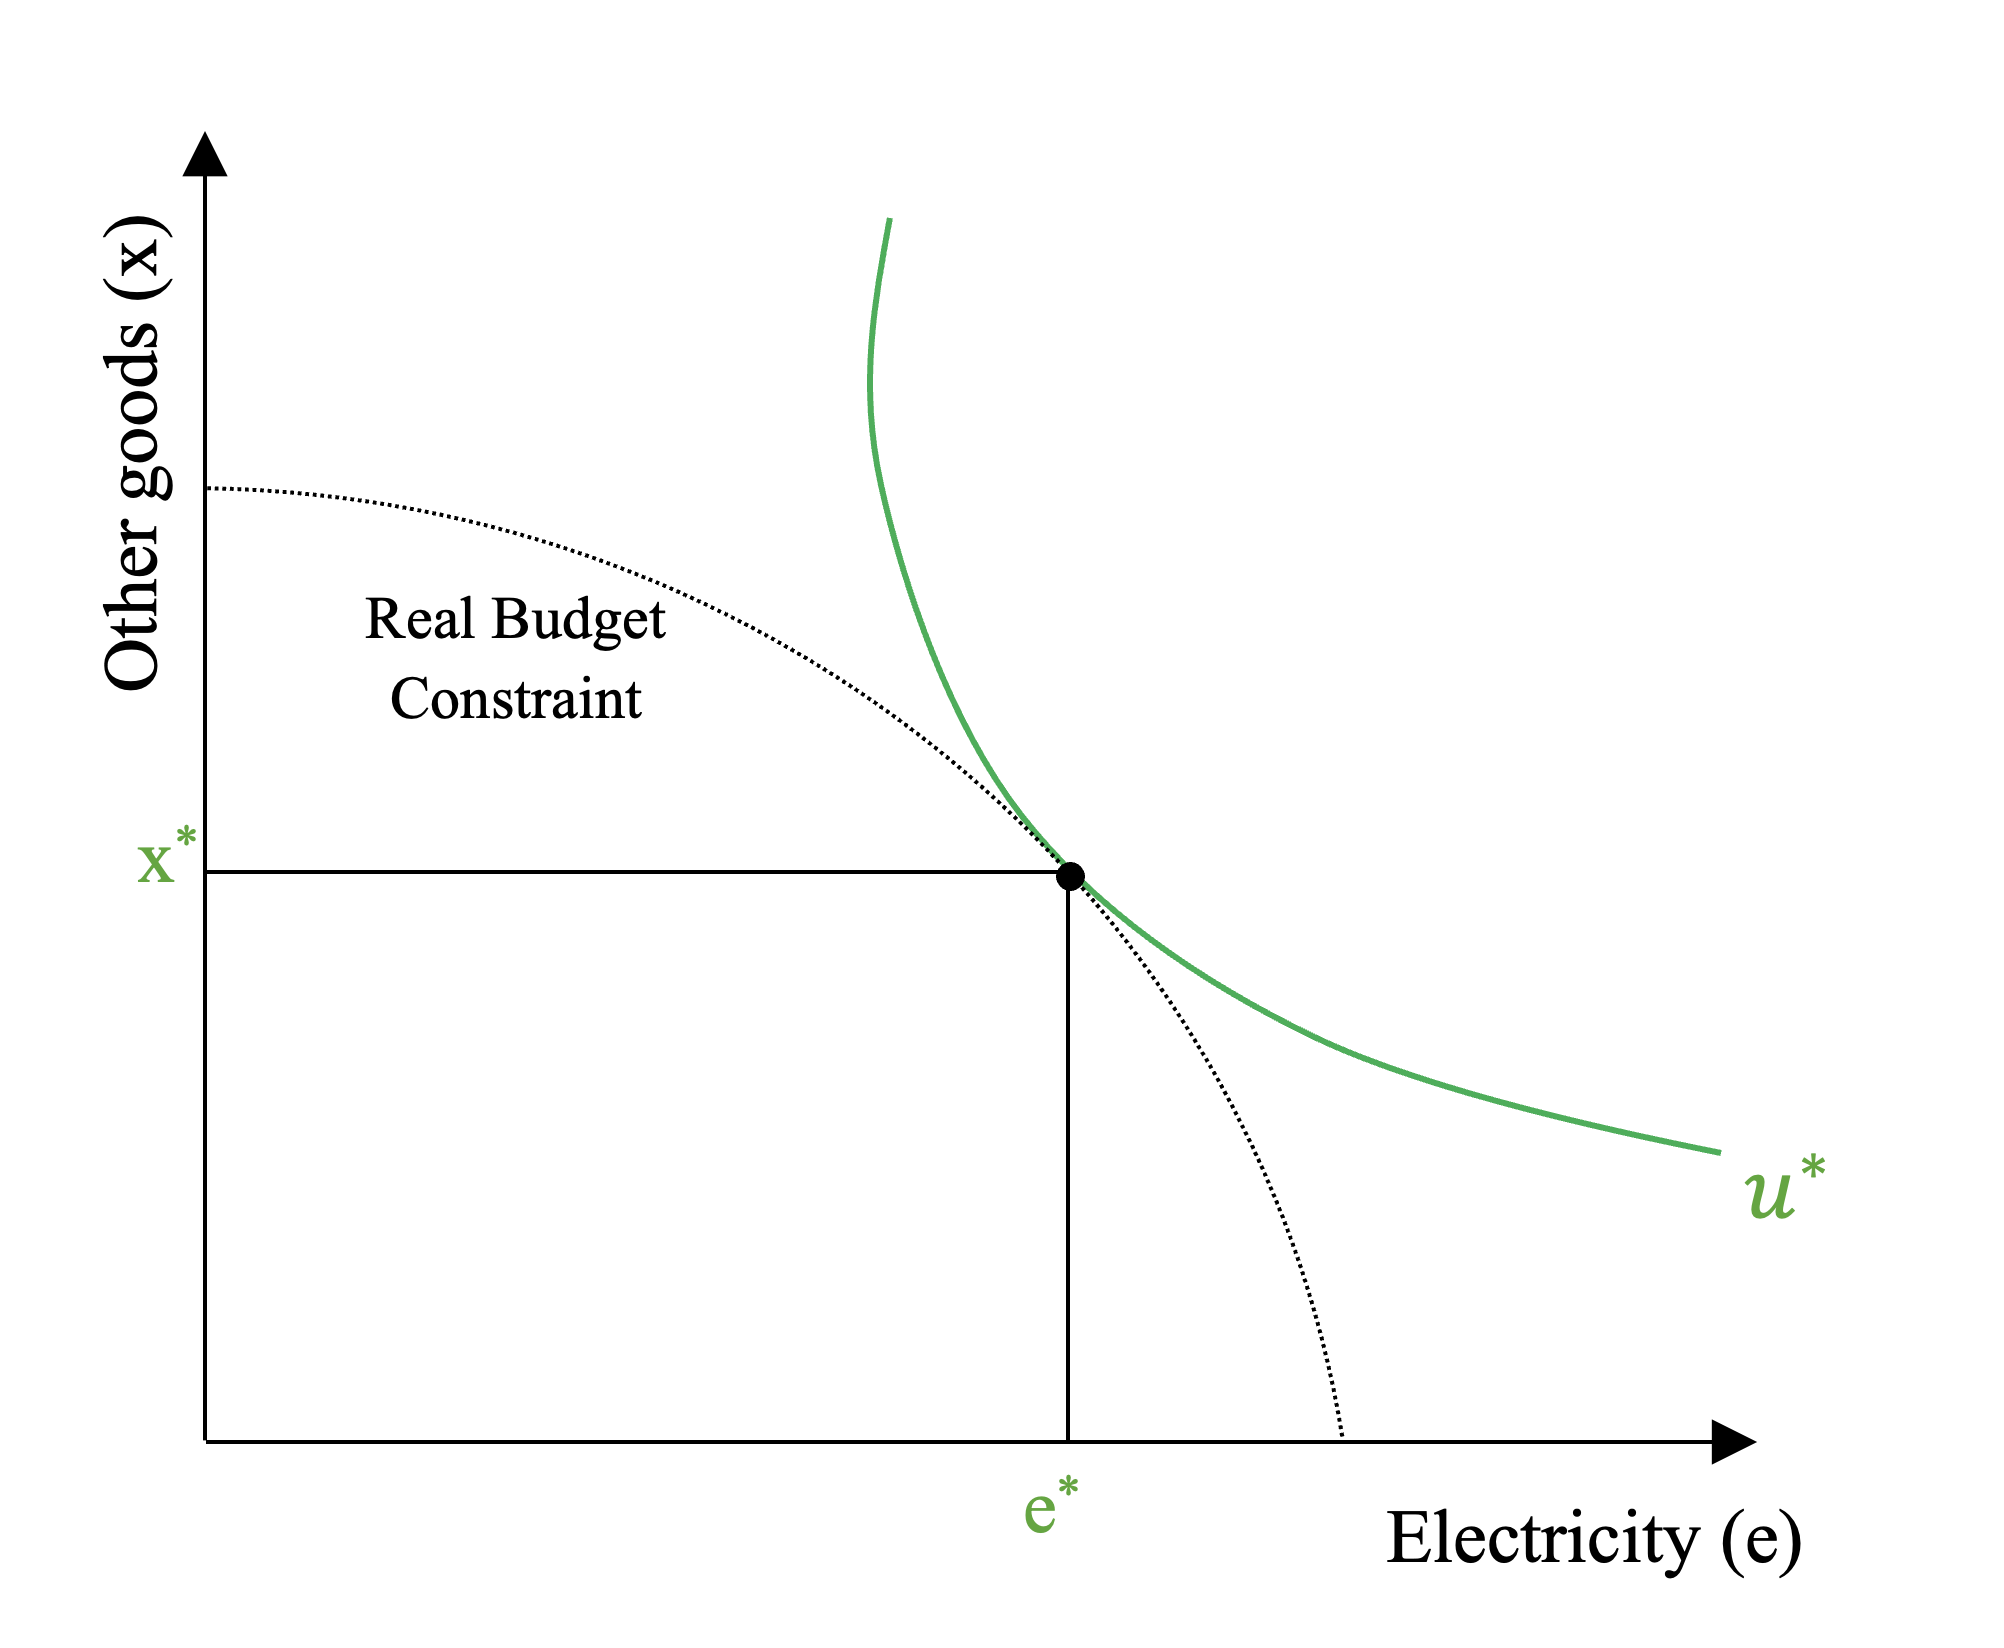
\includegraphics[width=\textwidth]{paper/figures/Theory_plot_a (1).png}
        \caption{Under rationality}
        \label{fig:Theory_a}
    \end{subfigure}
    
    \vspace{0.5cm}
    
    \begin{subfigure}[b]{0.75\textwidth}
        \centering
        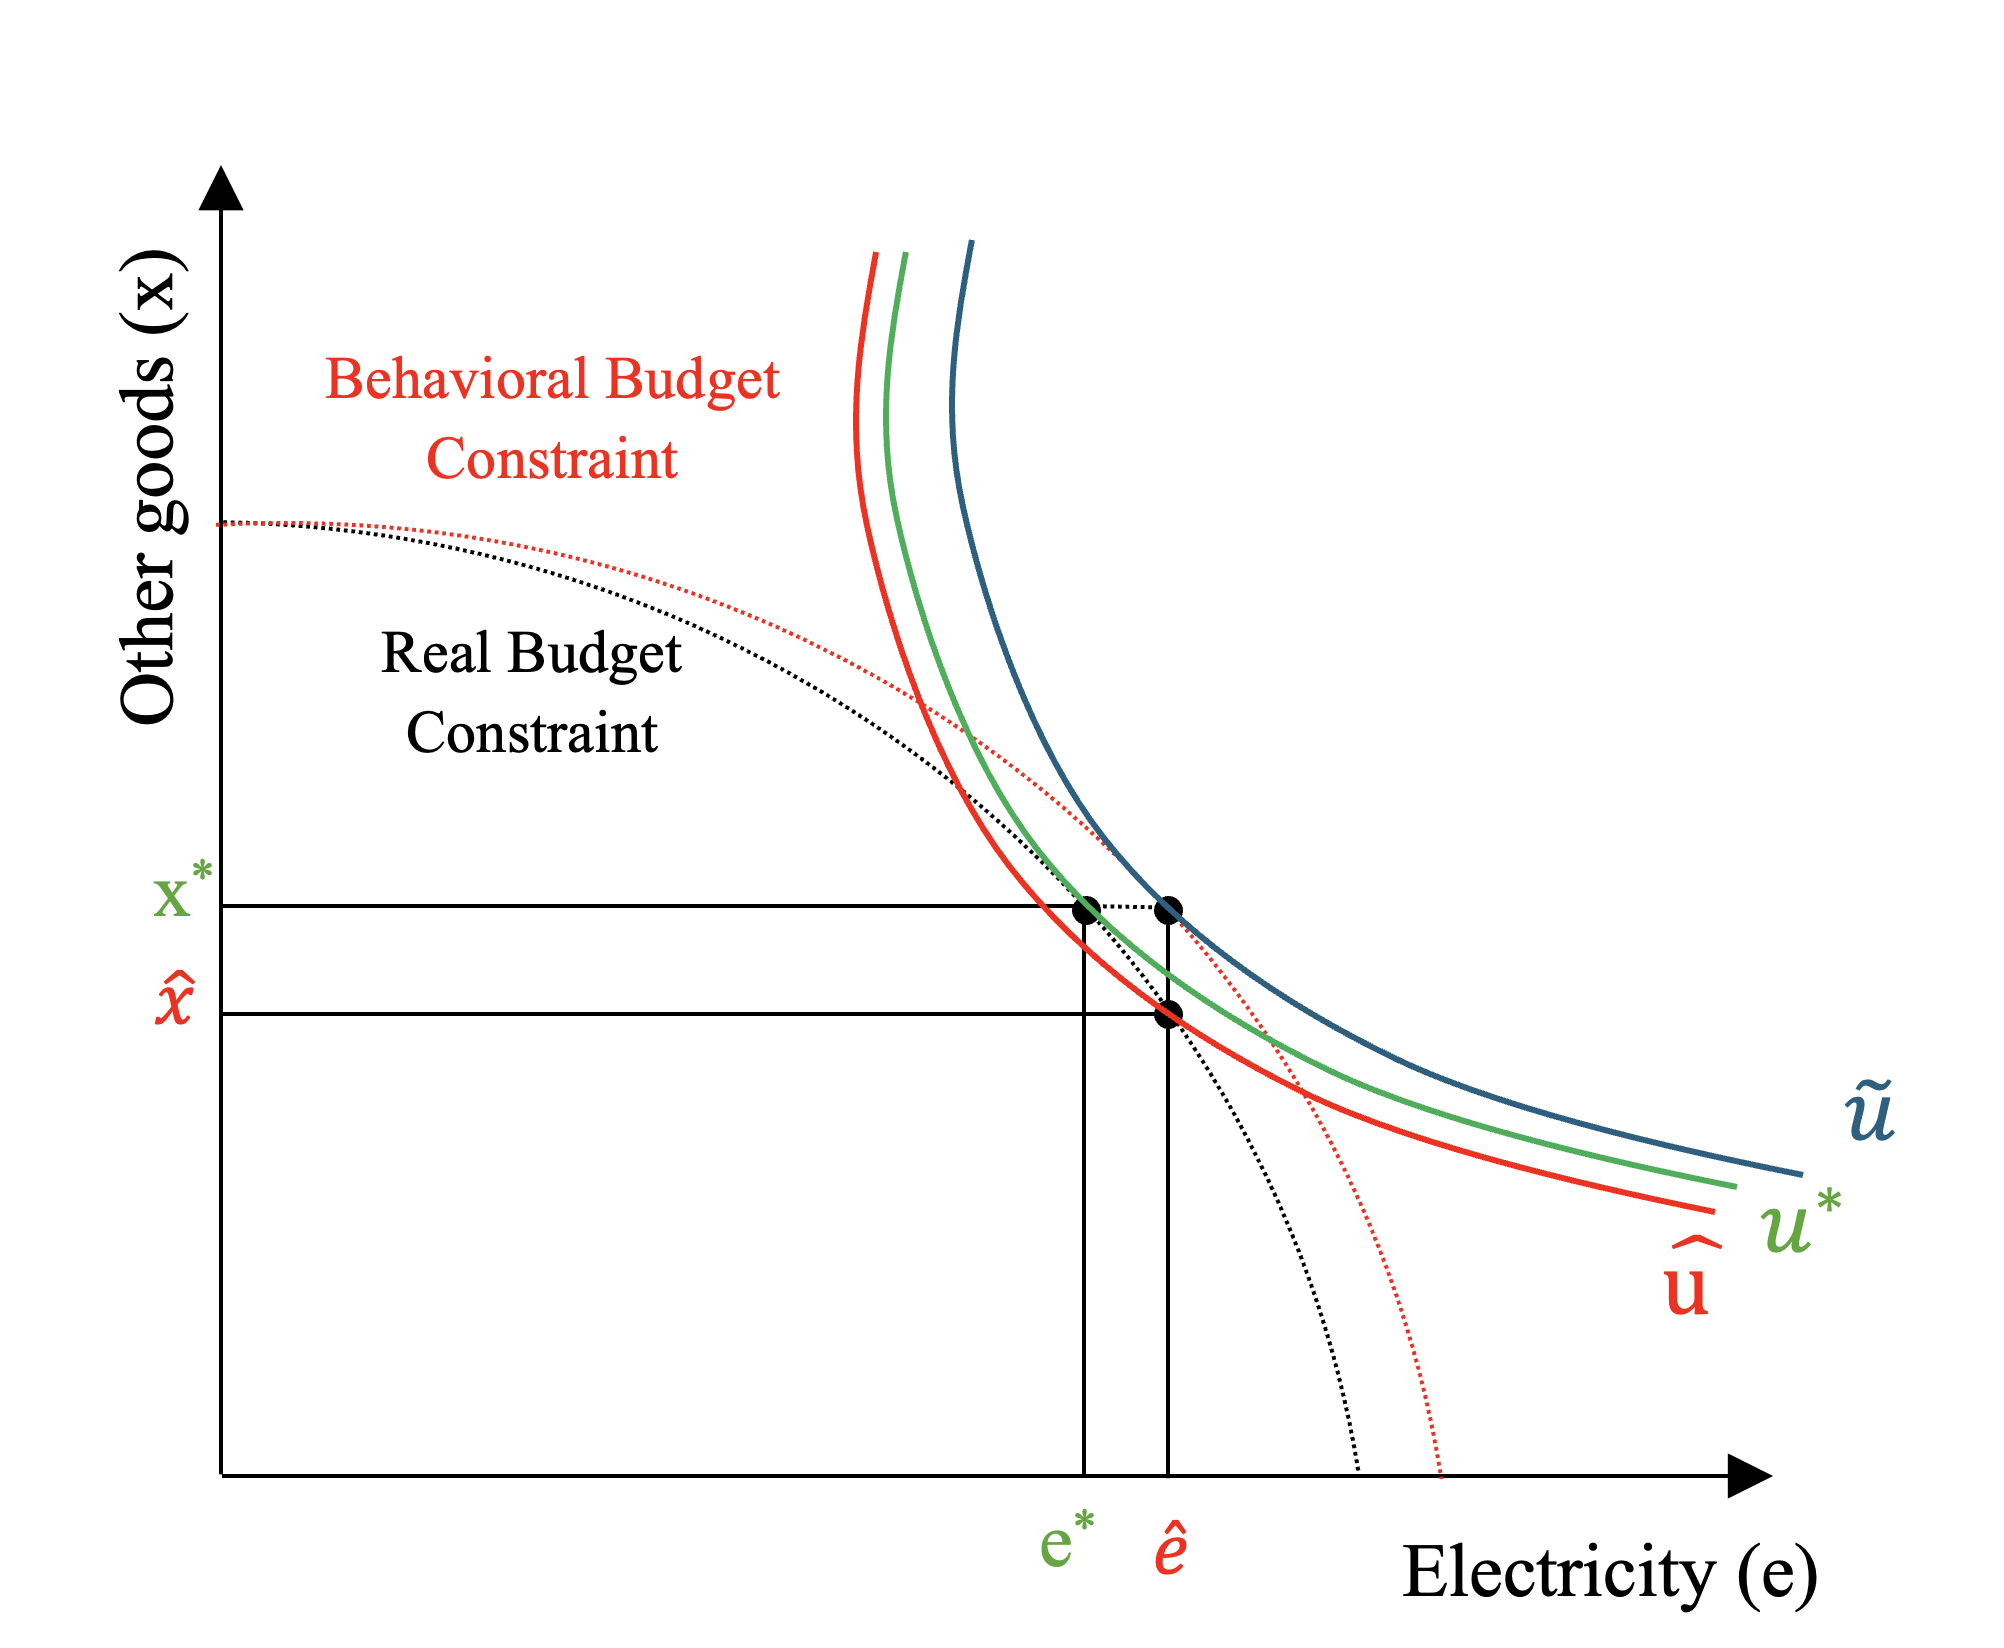
\includegraphics[width=\textwidth]{paper/figures/Theory plot b (1).png}
        \caption{Under bounded rationality (salience bias)}
        \label{fig:Theory_b}
    \end{subfigure}
    \caption{Illustration of the effects of salience bias on household consumption decisions. Adapted from \citet{alcocerSalienceBiasFramework2024}.}
     \label{fig:Theory}
\end{figure}

\subsection{Behavioral Extension: Salience Bias}

We generalize the neoclassical setup by assuming there are two relevant budget constraints. The first is the real constraint \( F(x, e) = 0 \), which always holds. Under bounded rationality, there is also a behavioral budget constraint, which the agent mistakenly follows first:
\[
F(x, e) := F(x, \tau e) = 0,
\]
where \( e \) is the \emph{behavioral good}. It is salience-prone and, accordingly, its current consumption is not always prominent. This generates a behavioral bias. The other good, \( x \), generates no salience bias, and the consumer is perfectly aware of its impact on her budget. We introduce \( \tau \in (0, 1] \), a parameter capturing the salience of electricity's consumption level and price. When electricity is not salient, households underestimate its marginal cost, which can be formalized as an attenuation in the perceived price, i.e., acting as if the cost were \( \tau p_e \) with \( \tau < 1 \). This salience bias leads to overconsumption relative to the neoclassical benchmark. Although the framework can be generalized to allow \( \tau \in (0, \infty) \) or multiple behavioral goods, we restrict attention to \( \tau \in (0,1] \), which captures the empirically observed tendency to underweight non-salient goods like electricity \citep[see]{tiefenbeck_overcoming_2018,alcocer_salience_2024}. \\

Given the salience distortion, the agent behaves as if the cost of electricity is \( \tau p_e \), with \( \tau < 1 \). The perceived (behavioral) budget constraint becomes:
\[
\tau p_e e + p_x x \leq w.
\]
Under this distorted perception, the agent maximizes utility:
\[
\max_{(e, x)} \quad u(e, x) \quad \text{s.t.} \quad \tau p_e e + p_x x \leq w.
\]
Let the solution be \( (\tilde{e}, \tilde{x}) \). Because electricity is underpriced in the agent’s perception (\( \tau < 1 \)), the resulting consumption choice will typically satisfy \( \tilde{e} > e^* \) and \( \tilde{x} < x^* \), leading to lower overall utility: \( u(\tilde{e}, \tilde{x}) < u(e^*, x^*) \).\footnote{Formally, this follows from the strict quasiconcavity of \( u(e, x) \) and the fact that both the real and behavioral budget constraints are linear and binding. The salience bias effectively rotates the perceived budget constraint outward along the electricity axis, inducing overconsumption of \( e \) and underconsumption of \( x \). Since \( (\tilde{e}, \tilde{x}) \) lies on a lower indifference curve than \( (e^*, x^*) \), utility must decline. For a formal proof, see \citet[Appendix A.1]{alcocer_salience_2024}.} \\ 

Figure~\ref{fig:Theory_b} illustrates this mechanism. In the benchmark case where electricity costs are fully salient (\( \tau = 1 \)), the agent chooses the utility-maximizing bundle \( (e^*, x^*) \) on the real budget constraint, reaching the highest feasible indifference curve \( u^* \). By contrast, when electricity is underweighted due to salience bias (\( \tau < 1 \)), the agent initially optimizes under a distorted budget constraint, leading to the selection of a biased consumption bundle \( (\hat{e}, \hat{x}) \). Once the true constraint is realized, she must reduce consumption of other goods to \( \tilde{x} < x^* \), while electricity consumption remains elevated at \( \hat{e} > e^* \). The final bundle \( (\hat{e}, \tilde{x}) \) lies on a lower indifference curve \( \hat{u} \), illustrating that the salience bias reduces overall utility. TThis unattainable indifference curve \( \tilde{u} \), corresponding to the perceived utility under the behavioral constraint, was never within the actual choice set. \\


Importantly, the salience parameter \( \tau \) is not fixed. It can be increased by interventions that raise the visibility of consumption and costs. In our experimental design, we deliver personalized, high-frequency feedback via a mobile app. This increases the salience of electricity use, thereby correcting the perceived budget distortion. The agent could thereby reduce the bias in the perceived constraint and improve welfare.

Let \( \tau_t \) denote the salience parameter at time \( t \), which increases with continued feedback and learning:
\[
\tau_{t+1} > \tau_t, \quad \lim_{t \to \infty} \tau_t = 1.
\]

As the salience distortion fades (\( \tau_t \to 1 \)), consumption choices converge to the rational benchmark:
\[
\lim_{t \to \infty} (\tilde{e}_t, \tilde{x}_t) = (e^*, x^*),
\]
and utility increases accordingly. Thus, our model predicts that feedback interventions should reduce electricity consumption over time and raise household utility, provided they effectively increase the salience of cost.



